
        \documentclass[tikz]{standalone}
        \usepackage{tikz}
        \usetikzlibrary{trees,shapes.geometric,positioning}
        
        \begin{document}
        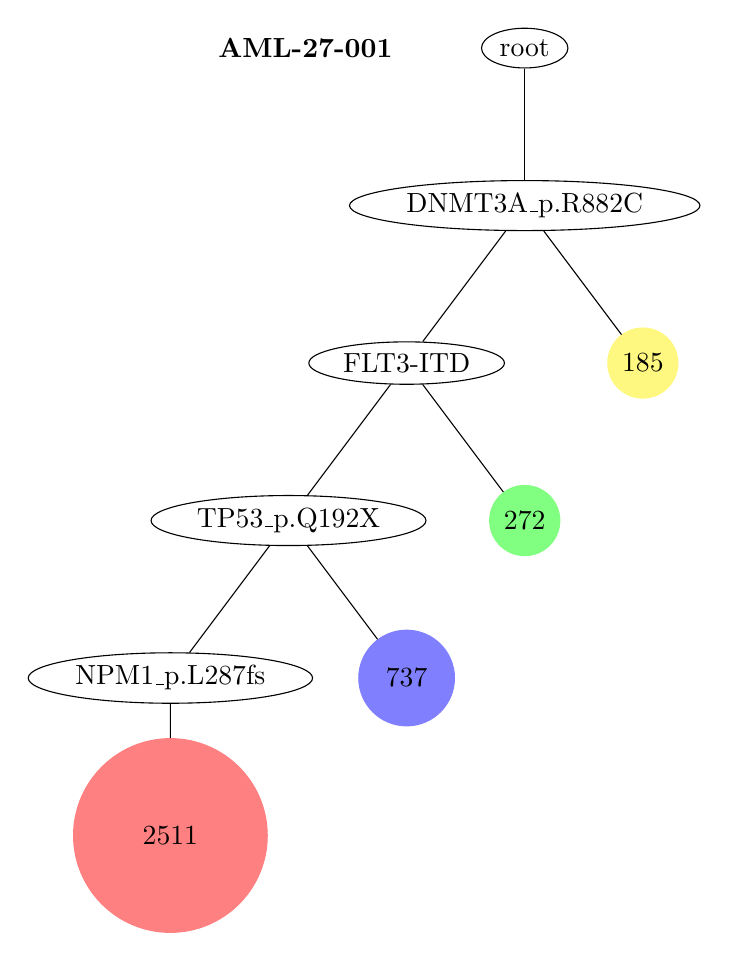
\begin{tikzpicture}[
            sizenode/.style 2 args={circle, draw=#1, fill=#1, minimum size=#2},
            treenode/.style={ellipse, draw, inner sep=2pt, align=center},
            level 1/.style={level distance=2cm,sibling distance=3cm},
            level 2/.style={level distance=2cm,sibling distance=3cm}
        ]
        
        \node [treenode] (root) {root}
	child {node [treenode] {DNMT3A\_p.R882C}
		child {node [treenode] {FLT3-ITD}
			child {node [treenode] {TP53\_p.Q192X}
				child {node [treenode] {NPM1\_p.L287fs}
					child {node [sizenode={red!50}{2.4594316186372973cm}] {2511}}
				}
				child {node [sizenode={blue!50}{1.2146150707447285cm}] {737}}
			}
			child {node [sizenode={green!50}{0.5728462144050996cm}] {272}}
		}
		child {node [sizenode={yellow!50}{0.4130970887094085cm}] {185}}
	};

\node [left=1cm of root] {\textbf{AML-27-001}};


        \end{tikzpicture}
        \end{document}
        